
\documentclass[letterpaper,hide notes,xcolor={table,svgnames},pdftex,10pt]{beamer}
\def\showexamples{t}

\usecolortheme{crane}
\setbeamertemplate{navigation symbols}{}

\usetheme{MyPittsburgh}
\usepackage{hyperref}
\usepackage{graphicx,xspace}
\usepackage[normalem]{ulem}
\usepackage{multicol}
\usepackage{amsmath,amssymb,amsthm,graphicx,xspace}
\newcommand\SF[1]{$\bigstar$\footnote{SF: #1}}

\usepackage[sfdefault,lf]{carlito}
\usepackage[T1]{fontenc}
\usepackage[scaled]{beramono}
\usepackage{tikzpagenodes}
\newcommand{\Rplus}{\protect\hspace{-.1em}\protect\raisebox{.35ex}{\small{\small\textbf{+}}}}
\newcommand{\Cpp}{\mbox{C\Rplus\Rplus}\xspace}

\newcounter{tmpnumSlide}
\newcounter{tmpnumNote}

\newcommand\mnote[1]{%
	\addtocounter{tmpnumSlide}{1}
	\ifdefined\showcues {~\tiny\fbox{\arabic{tmpnumSlide}}}\fi
	\note{\setlength{\parskip}{1ex}\addtocounter{tmpnumNote}{1}\textbf{\Large \arabic{tmpnumNote}:} {#1\par}}}

\newcommand\mmnote[1]{\note{\setlength{\parskip}{1ex}#1\par}}


\newcommand\mquestion[2]{{~\color{red}\fbox{?}}\note{\setlength{\parskip}{1ex}\par{\Large \textbf{?}} #1} \note{\setlength{\parskip}{1ex}\par{\Large \textbf{A}} #2\par}\ifdefined \presentationonly \pause \fi}

\newcommand\blackboard[1]{%
	\ifdefined   \showblackboard
		{#1}
	\else {\begin{center} \fbox{\colorbox{blue!30}{%
						\begin{minipage}{.95\linewidth}%
							\hspace{\stretch{1}} Some space intentionally left blank; done at the blackboard.%
						\end{minipage}}}\end{center}}%
	\fi%
}

\usepackage{listings}
\lstset{%
	keywordstyle=\bfseries,
	aboveskip=15pt,
	belowskip=15pt,
	captionpos=b,
	identifierstyle=\ttfamily,
	frame=lines,
	numbers=left, basicstyle=\scriptsize, numberstyle=\tiny, stepnumber=0, numbersep=2pt}

\usepackage{siunitx}
\newcommand\sius[1]{\num[group-separator = {,}]{#1}\si{\micro\second}}
\newcommand\sims[1]{\num[group-separator = {,}]{#1}\si{\milli\second}}
\newcommand\sins[1]{\num[group-separator = {,}]{#1}\si{\nano\second}}
\sisetup{group-separator = {,}, group-digits = true}

%% -------------------- tikz --------------------
\usepackage{tikz}
\usetikzlibrary{positioning}
\usetikzlibrary{arrows,backgrounds,automata,decorations.shapes,decorations.pathmorphing,decorations.markings,decorations.text}

\tikzstyle{place}=[circle,draw=blue!50,fill=blue!20,thick, inner sep=0pt,minimum size=6mm]
\tikzstyle{transition}=[rectangle,draw=black!50,fill=black!20,thick, inner sep=0pt,minimum size=4mm]

\tikzstyle{block}=[rectangle,draw=black, thick, inner sep=5pt]
\tikzstyle{bullet}=[circle,draw=black, fill=black, thin, inner sep=2pt]

\tikzstyle{pre}=[<-,shorten <=1pt,>=stealth',semithick]
\tikzstyle{post}=[->,shorten >=1pt,>=stealth',semithick]
\tikzstyle{bi}=[<->,shorten >=1pt,shorten <=1pt, >=stealth',semithick]

\tikzstyle{mut}=[-,>=stealth',semithick]

\tikzstyle{treereset}=[dashed,->, shorten >=1pt,>=stealth',thin]

\usepackage{ifmtarg}
\usepackage{xifthen}
\makeatletter
% new counter to now which frame it is within the sequence
\newcounter{multiframecounter}
% initialize buffer for previously used frame title
\gdef\lastframetitle{\textit{undefined}}
% new environment for a multi-frame
\newenvironment{multiframe}[1][]{%
	\ifthenelse{\isempty{#1}}{%
		% if no frame title was set via optional parameter,
		% only increase sequence counter by 1
		\addtocounter{multiframecounter}{1}%
	}{%
		% new frame title has been provided, thus
		% reset sequence counter to 1 and buffer frame title for later use
		\setcounter{multiframecounter}{1}%
		\gdef\lastframetitle{#1}%
	}%
	% start conventional frame environment and
	% automatically set frame title followed by sequence counter
	\begin{frame}%
		\frametitle{\lastframetitle~{\normalfont(\arabic{multiframecounter})}}%
		}{%
	\end{frame}%
}
\makeatother

\makeatletter
\newdimen\tu@tmpa%
\newdimen\ydiffl%
\newdimen\xdiffl%
\newcommand\ydiff[2]{%
	\coordinate (tmpnamea) at (#1);%
	\coordinate (tmpnameb) at (#2);%
	\pgfextracty{\tu@tmpa}{\pgfpointanchor{tmpnamea}{center}}%
	\pgfextracty{\ydiffl}{\pgfpointanchor{tmpnameb}{center}}%
	\advance\ydiffl by -\tu@tmpa%
}
\newcommand\xdiff[2]{%
	\coordinate (tmpnamea) at (#1);%
	\coordinate (tmpnameb) at (#2);%
	\pgfextractx{\tu@tmpa}{\pgfpointanchor{tmpnamea}{center}}%
	\pgfextractx{\xdiffl}{\pgfpointanchor{tmpnameb}{center}}%
	\advance\xdiffl by -\tu@tmpa%
}
\makeatother
\newcommand{\copyrightbox}[3][r]{%
	\begin{tikzpicture}%
		\node[inner sep=0pt,minimum size=2em](ciimage){#2};
		\usefont{OT1}{phv}{n}{n}\fontsize{4}{4}\selectfont
		\ydiff{ciimage.south}{ciimage.north}
		\xdiff{ciimage.west}{ciimage.east}
		\ifthenelse{\equal{#1}{r}}{%
			\node[inner sep=0pt,right=1ex of ciimage.south east,anchor=north west,rotate=90]%
			{\raggedleft\color{black!50}\parbox{\the\ydiffl}{\raggedright{}#3}};%
		}{%
			\ifthenelse{\equal{#1}{l}}{%
				\node[inner sep=0pt,right=1ex of ciimage.south west,anchor=south west,rotate=90]%
				{\raggedleft\color{black!50}\parbox{\the\ydiffl}{\raggedright{}#3}};%
			}{%
				\node[inner sep=0pt,below=1ex of ciimage.south west,anchor=north west]%
				{\raggedleft\color{black!50}\parbox{\the\xdiffl}{\raggedright{}#3}};%
			}
		}
	\end{tikzpicture}
}


%% --------------------

%\usepackage[excludeor]{everyhook}
%\PushPreHook{par}{\setbox0=\lastbox\llap{MUH}}\box0}

%\vspace*{\stretch{1}

%\setbox0=\lastbox \llap{\textbullet\enskip}\box0}

\setlength{\parskip}{\fill}

\newcommand\noskips{\setlength{\parskip}{1ex}}
\newcommand\doskips{\setlength{\parskip}{\fill}}

\newcommand\xx{\par\vspace*{\stretch{1}}\par}
\newcommand\xxs{\par\vspace*{2ex}\par}
\newcommand\tuple[1]{\langle #1 \rangle}
\newcommand\code[1]{{\sf \footnotesize #1}}
\newcommand\ex[1]{\uline{Example:} \ifdefined \presentationonly \pause \fi
	\ifdefined\showexamples#1\xspace\else{\uline{\hspace*{2cm}}}\fi}

\newcommand\ceil[1]{\lceil #1 \rceil}


\AtBeginSection[]
{
	\begin{frame}
		\frametitle{Outline}
		\tableofcontents[currentsection]
	\end{frame}
}



\pgfdeclarelayer{edgelayer}
\pgfdeclarelayer{nodelayer}
\pgfsetlayers{edgelayer,nodelayer,main}

\tikzstyle{none}=[inner sep=0pt]
\tikzstyle{rn}=[circle,fill=Red,draw=Black,line width=0.8 pt]
\tikzstyle{gn}=[circle,fill=Lime,draw=Black,line width=0.8 pt]
\tikzstyle{yn}=[circle,fill=Yellow,draw=Black,line width=0.8 pt]
\tikzstyle{empty}=[circle,fill=White,draw=Black]
\tikzstyle{bw} = [rectangle, draw, fill=blue!20,
text width=4em, text centered, rounded corners, minimum height=2em]

\newcommand{\CcNote}[1]{% longname
	This work is licensed under the \textit{Creative Commons #1 3.0 License}.%
}
\newcommand{\CcImageBy}[1]{%
	\includegraphics[scale=#1]{creative_commons/cc_by_30.pdf}%
}
\newcommand{\CcImageSa}[1]{%
	\includegraphics[scale=#1]{creative_commons/cc_sa_30.pdf}%
}
\newcommand{\CcImageNc}[1]{%
	\includegraphics[scale=#1]{creative_commons/cc_nc_30.pdf}%
}
\newcommand{\CcGroupBySa}[2]{% zoom, gap
	\CcImageBy{#1}\hspace*{#2}\CcImageNc{#1}\hspace*{#2}\CcImageSa{#1}%
}
\newcommand{\CcLongnameByNcSa}{Attribution-NonCommercial-ShareAlike}

\newenvironment{changemargin}[1]{% 
	\begin{list}{}{% 
		\setlength{\topsep}{0pt}% 
		\setlength{\leftmargin}{#1}% 
		\setlength{\rightmargin}{1em}
		\setlength{\listparindent}{\parindent}% 
		\setlength{\itemindent}{\parindent}% 
		      \setlength{\parsep}{\parskip}% 
		      }% 
		\item[]}{\end{list}}




\title{Lecture 11 --- Threads}

\author{Jeff Zarnett \\ \small \texttt{jzarnett@uwaterloo.ca}}
\institute{Department of Electrical and Computer Engineering \\
	University of Waterloo}
\date{\today}


\begin{document}

\begin{frame}
	\titlepage

\end{frame}

\begin{frame}
	\frametitle{What is a Thread?}


	Recall our earlier examination of the process.

	A process has three major components:
	\begin{enumerate}
		\item An executable program;
		\item The data created/needed by the program; and
		\item The execution context of the program.
	\end{enumerate}

	A process has at least one \alert{thread}, and can have many.

\end{frame}

\begin{frame}
	\frametitle{What is a Thread?}

	The term ``thread'' is a short form of \alert{Thread of Execution}.

	A thread of execution is a sequence of executable commands that can be scheduled to run on the CPU.

	Threads also have some state and stores some local variables.

	Most programs you will write in other courses have only one thread;\\
	\quad that is, your program's code is executed one statement at a time.

\end{frame}

\begin{frame}
	\frametitle{Multithreaded Programs}

	A multithreaded program uses more than one thread, (some of the time).

	A program begins with an initial thread (where the \texttt{main} method is).

	That main thread can create some additional threads if needed.

	Threads can be created and destroyed within a program dynamically.

\end{frame}

\begin{frame}
	\frametitle{Threads and Processes}

	\begin{center}
		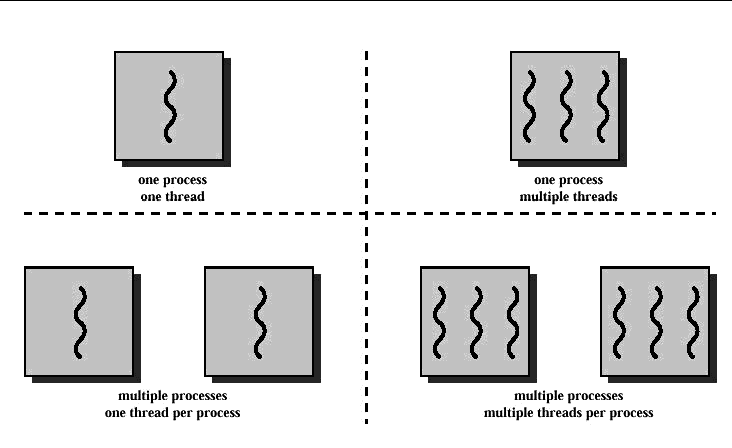
\includegraphics[width=0.9\textwidth]{images/mthread.png}
	\end{center}

\end{frame}

\begin{frame}
	\frametitle{Thread Possessions}


	In a process that has multiple threads, each thread has its own:
	\begin{enumerate}
		\item Thread execution state.
		\item Saved thread context when not running.
		\item Execution stack.
		\item Local variables.
		\item Access to the memory and resources of the process (shared with all threads in that process).
	\end{enumerate}

\end{frame}

\begin{frame}
	\frametitle{Single vs. Multithreaded}

	\begin{center}
		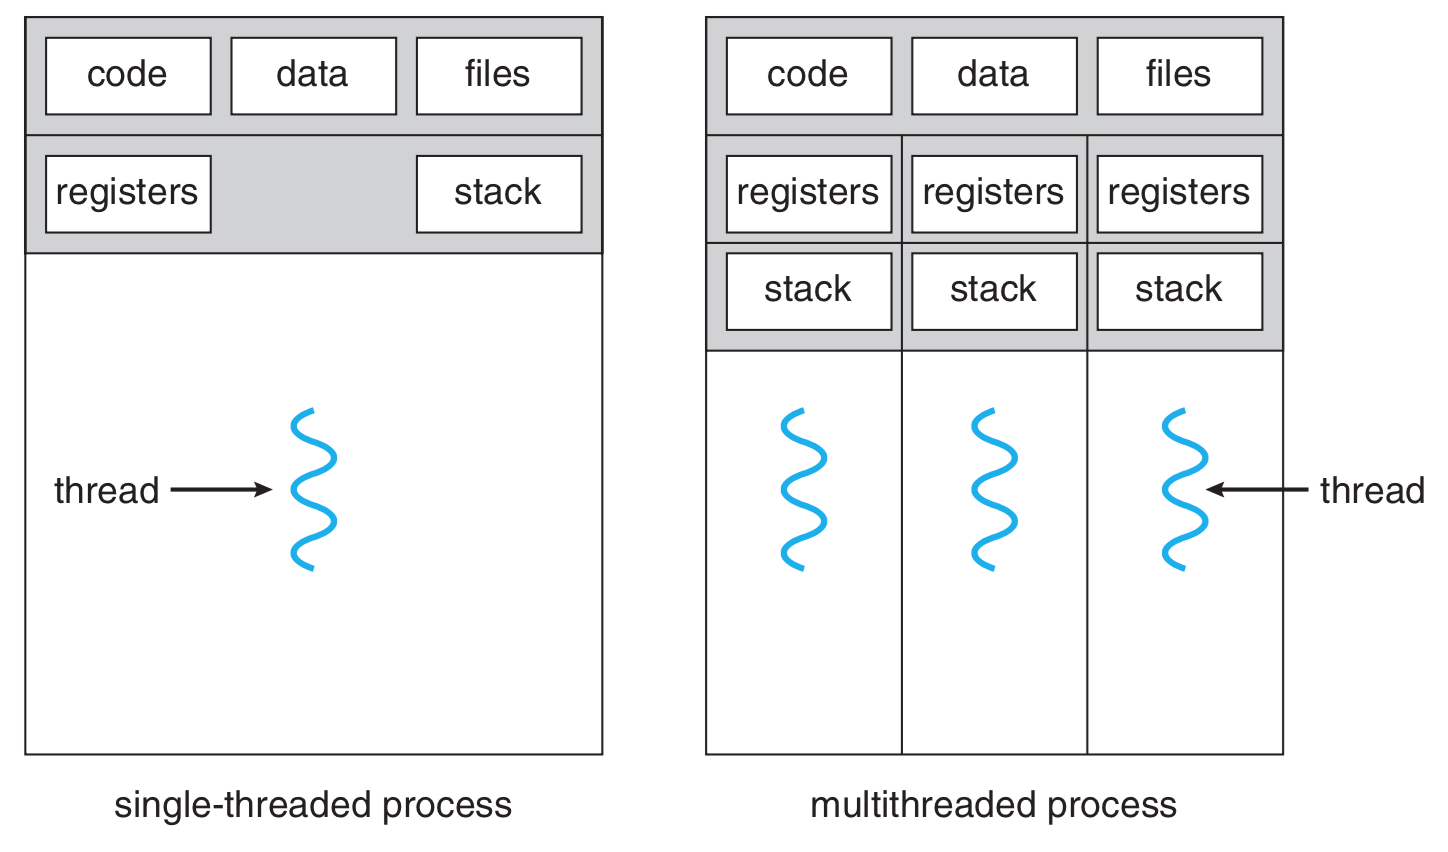
\includegraphics[width=0.9\textwidth]{images/mthread2.png}
	\end{center}

\end{frame}

\begin{frame}
	\frametitle{Thread Notes}

	All the threads of a process share the state and resources of the process.

	If a thread opens a file, other threads in that process can also access it.

	The way programs are written now, few are not multithreaded.



\end{frame}

\begin{frame}
	\frametitle{UI Thread}

	One common way of dividing up the program into threads is to separate the user interface from a time-consuming action.

	Consider a file-transfer program.

	If the user interface and upload method share a thread, once a file upload has started, the user will not be able to use the UI anymore.

	Not even to click the button that cancels the upload!

	For some reason, users hate that.

\end{frame}

\begin{frame}
	\frametitle{Solving the UI Thread Problem}

	We have two options for how to alleviate this problem.

	Option 1: \texttt{fork} a new process to do the upload; or \\
	Option 2: Spawn  new thread.

	In either case, the newly created entity will handle the upload of the file.

	The UI remains responsive, because the UI thread is not waiting for the upload method to complete.

\end{frame}

\begin{frame}
	\frametitle{Thread Motivation}
	Why threads instead of a new process?

	Primary motivation is: performance.

	\begin{enumerate}
		\item Creation: 10$\times$ faster.
		\item Terminating and cleaning up a thread is faster.
		\item Switch time: 20\% of process switch time.
		\item Shared memory space (no need for IPC).
		\item Lets the UI be responsive.
	\end{enumerate}

\end{frame}

\begin{frame}
	\frametitle{Common Usage of Threads}

	\begin{enumerate}
		\item \textbf{Foreground and Background Work}
		\item \textbf{Asynchronous processing}
		\item \textbf{Speed of Execution}
		\item \textbf{Modular Structure}
	\end{enumerate}

\end{frame}

\begin{frame}
	\frametitle{Thread Drawbacks}

	There is no protection between threads in the same process.

	One thread can easily mess with the memory being used by another.

	This once again brings us to the subject of co-ordination, which will follow the discussion of threads.

	Also, if any thread encounters an error, the whole process might be terminated by the operating system.

\end{frame}

\begin{frame}
	\frametitle{Thread States}
	Each individual thread will have its own state.

	Our process model has seven states.\\
	\quad The thread state model is the simpler five-state model.

	If a process is swapped out of memory, all its threads are swapped out.

	When that process returns to memory, all the threads are swapped in.

	Therefore we do not need to consider if a thread is in memory/swapped.

\end{frame}

\begin{frame}
	\frametitle{Five State Model}
	Five state model, once again:

	\begin{center}
		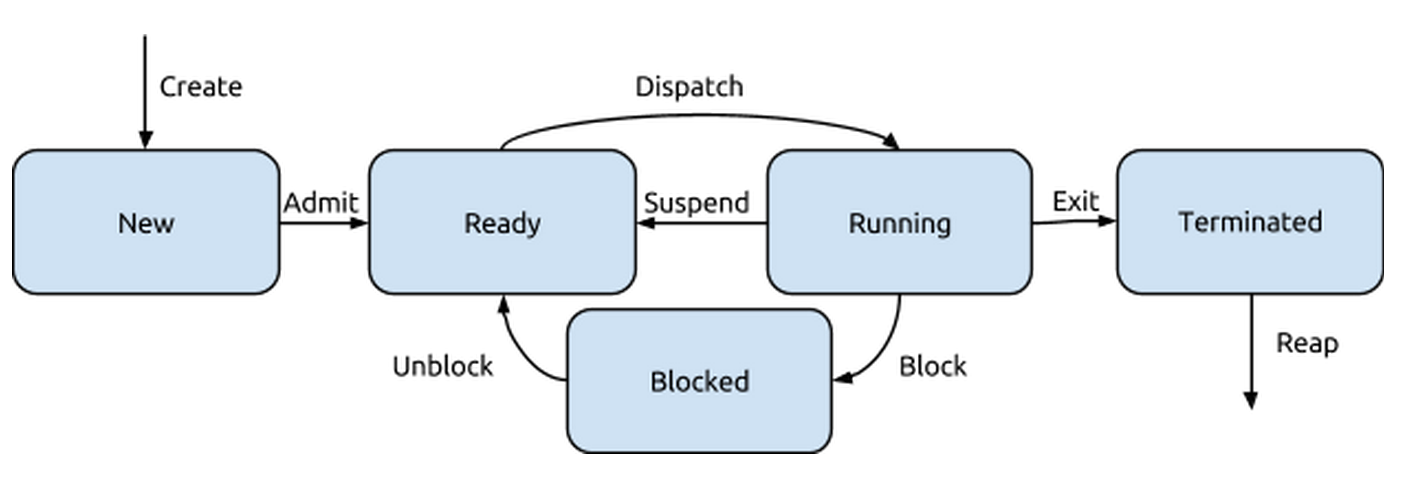
\includegraphics[width=0.85\textwidth]{images/5-state-model.png}
	\end{center}

\end{frame}

\begin{frame}
	\frametitle{Five State Model}

	The transitions work the same way as the state transitions for a process.

	As with a process, a thread in any state can transition to terminated.

	When a process is terminated, all its threads are terminated\\
	\quad Regardless of what state it is in.


\end{frame}


\begin{frame}
	\frametitle{The POSIX Thread}

	The term \texttt{pthread} refers to the POSIX standard (also known as the IEEE 1003.1c standard) that defines thread behaviour in UNIX.

	\begin{itemize}
		\item \texttt{pthread\_create}
		\item \texttt{pthread\_exit}
		\item \texttt{pthread\_join}
		\item \texttt{pthread\_detach}
		\item \texttt{pthread\_yield}
		\item \texttt{pthread\_attr\_init}
		\item \texttt{pthread\_attr\_destroy}
		\item \texttt{pthread\_cancel}
		\item \texttt{pthread\_testcancel}
	\end{itemize}

\end{frame}


\begin{frame}[fragile]
	\frametitle{Let's Make a New Thread}

	\begin{lstlisting}[language=C]
pthread_create( pthread_t *thread, 
		const pthread_attr_t * attr, 
		void *(*start_routine)( void * ), 
		void *arg);
\end{lstlisting}

	\texttt{thread}: a pointer to a \texttt{pthread} identifier and will be assigned a value when the thread is created.

	\texttt{attr}: attributes; may be \texttt{NULL} for defaults.

	\texttt{start\_routine}: the function the new thread is to run.

	\texttt{arg}: The argument passed to the routine we want to start.

\end{frame}


\begin{frame}[fragile]
	\frametitle{Start Routine}

	The type of \texttt{start\_routine} above is a function signature.

	Thus, the \texttt{pthread\_create} function has to be called with the name of a function matching that signature, such as:

	\begin{lstlisting}[language=C]
void* do_something( void* start_params )
\end{lstlisting}

	After creating a new thread, the process has two threads in it.

	Scheduling of the threads is up to the operating system.

\end{frame}


\begin{frame}[fragile]
	\frametitle{There Can Be Only One}

	C: it is normal to have a single return value from a function, but usually we can have multiple input parameters.

	But here we get only one of each?

	Define a \texttt{struct} for the argument and return type!

	\begin{lstlisting}[language=C]
void* function( void * void_arg ) {
  parameters_t *arguments = (parameters_t*) args;
  /* continue after this */
}
\end{lstlisting}

	We have to cast it inside the thread anyway...

	The caller of the \texttt{pthread\_create} function has to know what kind of argument is expected in the function being called.

\end{frame}


\begin{frame}
	\frametitle{Attributes}

	Attributes can be used to set whether a thread is detached or joinable, scheduling policy, etc.

	By default, new threads are usually joinable (that is to say, that some other thread can call \texttt{pthread\_join} on them).

	To prevent a thread from ever being joined, it can be created in the detached state (or use \texttt{pthread\_detach})

	For virtually all scenarios that we will consider in this course the default values will be fine.

\end{frame}

\begin{frame}
	\frametitle{Off We Go}

	The thread executes its function, until of course it gets to the end.

	Usually, it will terminate with \texttt{pthread\_exit}.

	The use of \texttt{pthread\_exit} is not the only way that a thread may be terminated.

	Sometimes we want the thread to persist (hang around), but if we want to get a return value from the thread, then we need it to exit.

\end{frame}


\begin{frame}
	\frametitle{Nobody's Listening}

	If a thread has no return values, it can just \texttt{return NULL;}

	This will send \texttt{NULL} back to the thread that has joined it.

	If the function that is called as a task returns normally rather than calling the exit routine, the thread will still be terminated.

\end{frame}

\begin{frame}
	\frametitle{Oh... Guess You Didn't Need This After All}

	Another way a thread might terminate is if the \texttt{pthread\_cancel} function.\\
	\quad We'll come back to this topic in more detail soon.

	A thread may also be terminated indirectly: if the entire process is terminated or if \texttt{main} finishes first (without calling \texttt{pthread\_exit} itself).

	End \texttt{main} with \texttt{pthread\_exit} to automatically wait for all spawned threads.

\end{frame}


\begin{frame}[fragile]
	\frametitle{Report, Number One!}

	Like the \texttt{wait} system call, the \texttt{pthread\_join} is how we get a value out of the spawned thread:

	\begin{lstlisting}[language=C]
pthread_join( pthread_t thread, void** retval );
\end{lstlisting}

	\texttt{thread}: the thread you wish to join.

	\texttt{retval}: wait... two stars?

\end{frame}

\begin{frame}
	\frametitle{Gotta Play the Level Again, Only Got 2 Stars}

	What we are looking for is a pointer to a void pointer.

	That is, we are going to supply a pointer that the join function will update to be pointing to the value returned by that function.

	Typically we supply the address of a pointer.

	Maybe the example makes it clearer.
\end{frame}


\begin{frame}[fragile]
	\frametitle{Collecting Return Value}

	\begin{lstlisting}[language=C]
#include <stdlib.h>
#include <stdio.h>
#include <pthread.h>

void * run( void * argument ) { 
  char* a = (char*) argument;
  printf("Provided argument is %s!\n", a); 
  int * return_val = malloc( sizeof( int )); 
  *return_val = 99; 
  pthread_exit( return_val );
}

int main( int argc, char** argv ) { 
  if (argc != 2) {
      printf("Invalid args.\n");
      return -1; 
  }
  pthread_t t;
  void* vr; 
  
  pthread_create( &t, NULL, run, argv[1] );
  pthread_join( t, &vr );
  int* r = (int*) vr; 
  printf("The other thread returned %d.\n", *r);
  free( vr );
  pthread_exit( 0 );
}
\end{lstlisting}


\end{frame}




\end{document}

